\section{Git - Sistema de control de versiones}

En esta sección se pide que se añadan capturas de pantalla mostrando los comandos git ejecutados para realizar las siguientes acciones:

\subsection{Creación de dos tags}

Se pide definir dos tags y se deja a criterio del estudiante en qué momento del proyecto realizarlos.

\begin{enumerate}
    \item El primer tag se ha creado cuando se ha conseguido una versión usable del código por primera vez. Se ha llamado \texttt{1.0}.

    \begin{center}
        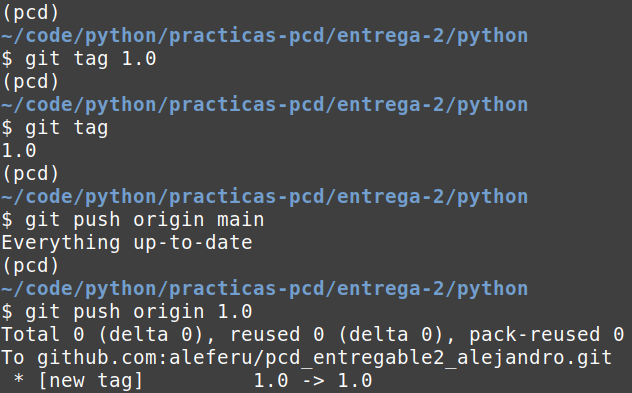
\includegraphics[width=0.7\textwidth]{img/tag1.png}
    \end{center}

    \newpage

    \item El segundo tag se ha creado cuando he terminado todo y estaba a punto de prepararlo todo para la entrega. Lo he llamado \texttt{entrega}.

    \begin{center}
        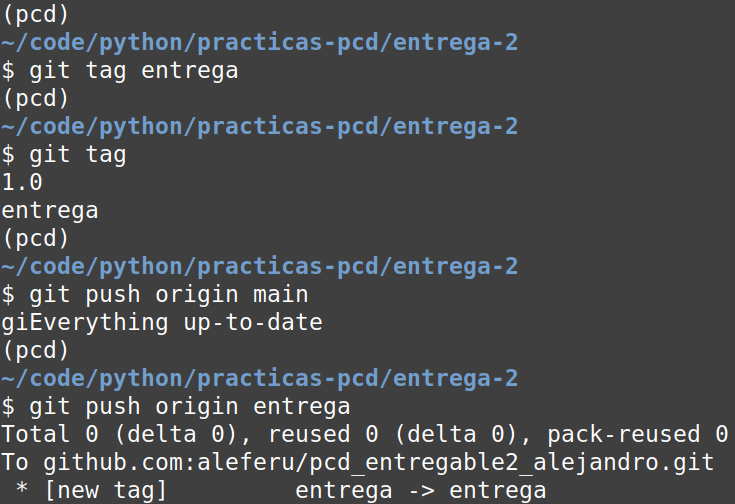
\includegraphics[width=0.7\textwidth]{img/tagentrega.png}
    \end{center}
\end{enumerate}


\subsection{Creación de un repositorio público en GitHub}

Se pide crear un repositorio público en GitHub que se llame \texttt{pcd\_entregable2\_alejandro} (en mi caso).

\begin{center}
    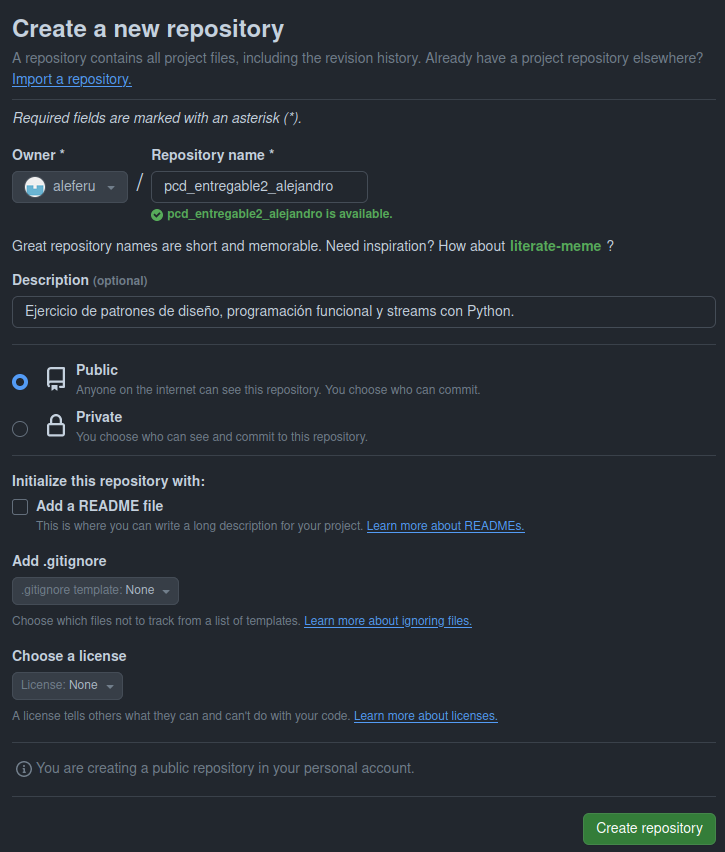
\includegraphics[width=0.68\textwidth]{img/creacion-repositorio-online.png}
\end{center}

Para enlazar el repositorio local y el online se ha utlizado el siguiente comando:

\begin{center}
    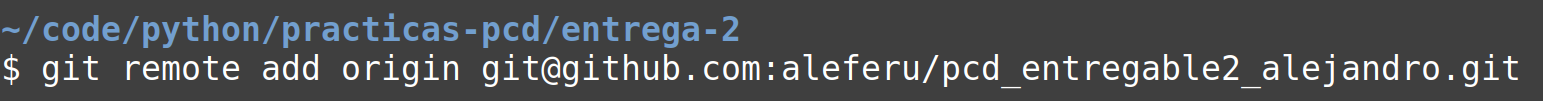
\includegraphics[width=0.7\textwidth]{img/repositorio-local-origin.png}
\end{center}
